\chapter{Implementation Details}
\label{chapter:eleven}

%The history of Scale Space tracks back to Witkin 1983, where it was applied to time series.  He highlighted the Spatial Coincidential assumption.
%Basically, the number of zero crossing of the first derivative is reduced with increasing scale.
%
%\begin{story}[Biomimetic Applications]
%
%\end{story}
%
%This method is actually composed on two submethods: the first is the keypoint localization, while the second is the histogram of gradient orientations, which is the basis for this thesis.
%
%bla bla bla
%
%
%Aca también voy a mandar detalles de la implementacion.   como por ejemplo los detalles de como funciona vlfeat y las modificaciones.


%\section{Implementation}
%
%\subsection{Software}
%
%The implemented code is published in \url{https://bitbucket.org/itba/hist/} by using Matlab, python and the VLFeat library.
%These algorithm were implemented on MATLAB 2014a (Mathworks Inc., Natick, MA, USA).  To maintain reproducibility, the data and the source code has been made available in the online repository of the Code Ocean platform under the name \textit{EEGWave}.
%
%The algorithm is implemented using  VLFeat~\cite{Vedaldi2010} Computer Vision libraries on MATLAB V2014a (Mathworks Inc., Natick, MA, USA). Furthermore, in order to enhance the impact of our paper and for a sake of reproducibility, the code of the algorithm has been made available at: https://bitbucket.org/itba/hist.

%TODO add the data and also the code ocean repository.  Also add my own repositories.


\section{Open Source Software}
The software produced for this Thesis can be found in the following public repositories:

\begin{itemize}
\item \url{https://bitbucket.org/itba/hist}
\item \url{https://github.com/faturita/BciVisualToolbox}
\item \url{https://github.com/faturita/vlfeat}
\item \url{https://github.com/faturita/GuessMe}
\end{itemize}

\section{Public Datasets}

\begin{itemize}
\item P300-Dataset \url{https://www.kaggle.com/rramele/p300samplingdataset}, Registered as public scientific resource in the public Database SciCrunch, RRID: SCR\_015977. 
\item P300 Template (routput.mat) and P300-null signal subject (P300-Subject-21.mat) at the CodeBase Repository \url{https://goo.gl/MzNNkn}.
\end{itemize}

\section{Blog and Online Resources}

\begin{itemize}
\item The following blog was mantained during the development of this Thesis: \url{http://monostuff.logdown.com/}.
\end{itemize}

\section{Keypoint Localization Details}

\begin{figure}[h!]
\centering
\subfigure[]
{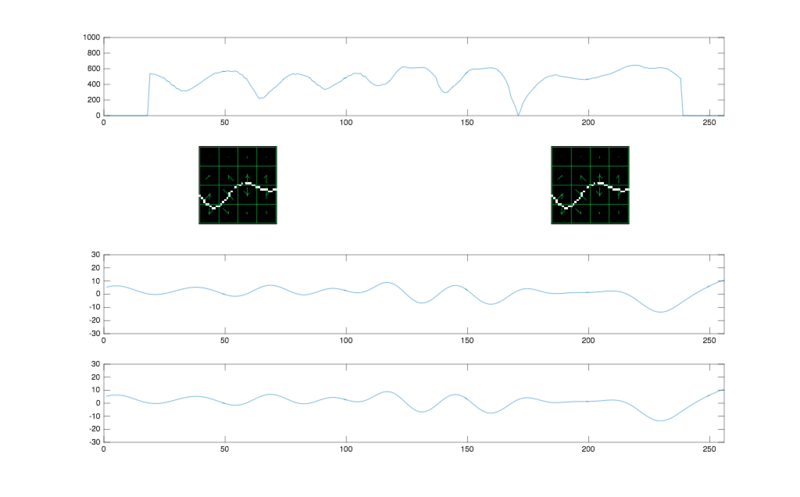
\includegraphics[scale=0.6]{images/dialdescriptores1.png}}
\caption[Patch localization on a nonmodified signal]{Upper panel shows the euclidean distance between the descriptor 1 obtained from the left patch, and descriptor 2 obtained from the right patch.  Lower panels show the signal 1, which is used to generate the first descriptor and signal 2 which is used to generate the patch from the right.  The signals are exactly the same, hence the distance between descriptors is zero at exactly the keypoint position.}
\label{fig:dialdescriptors1}
\end{figure}


\begin{figure}[h!]
\centering
\subfigure[]
{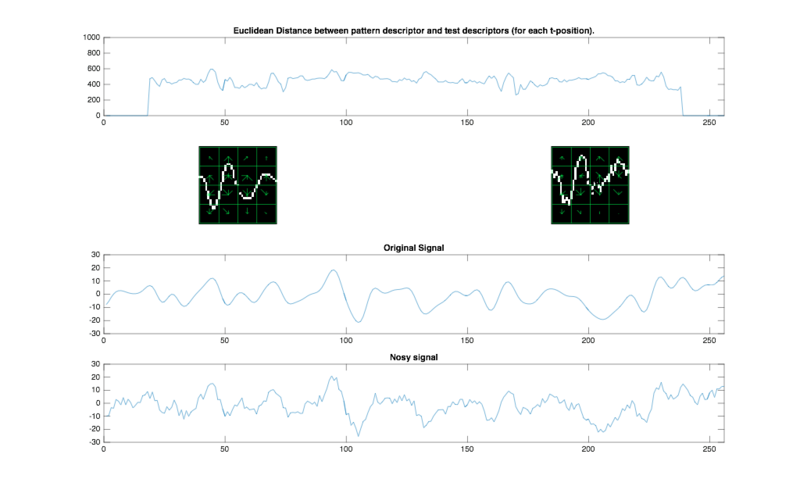
\includegraphics[scale=0.6]{images/dialdescriptores3.png}}
\caption[Patch localization on a noisy signal]{In this case, the signal from the bottom panel has a superimposed additive artificial random noise of $5 \si{db}$.  Although the minimum value is still the correct localization of the keypoint, there is a false positive which differs only $3\%$ of the real value. }
\label{fig:dialdescriptors1}
\end{figure}


\begin{figure}[h!]
\centering
\subfigure[]
{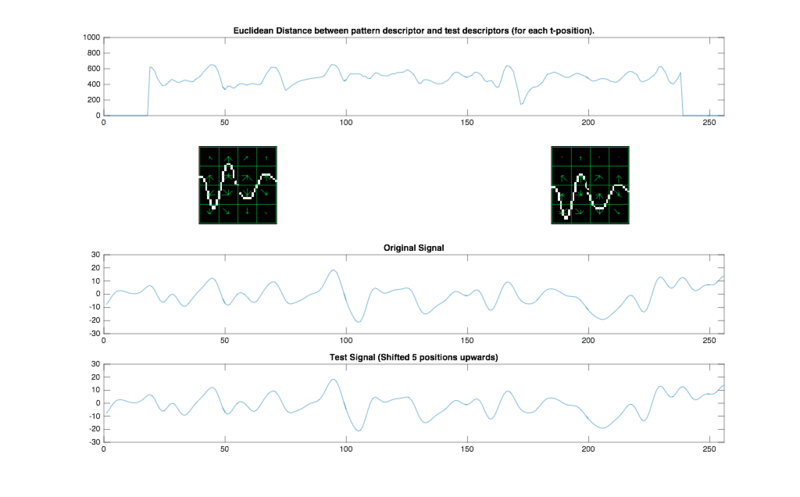
\includegraphics[scale=0.6]{images/dialdescriptores5.png}}
\caption[Patch localization on a vertical translated keypoint]{If the keypoint is vertically translated 5 pixels downward or upward, the keypoint can't no longer be identified correctly.}
\label{fig:dialdescriptors1}
\end{figure}


\begin{figure}[h!]
\centering
\subfigure[]
{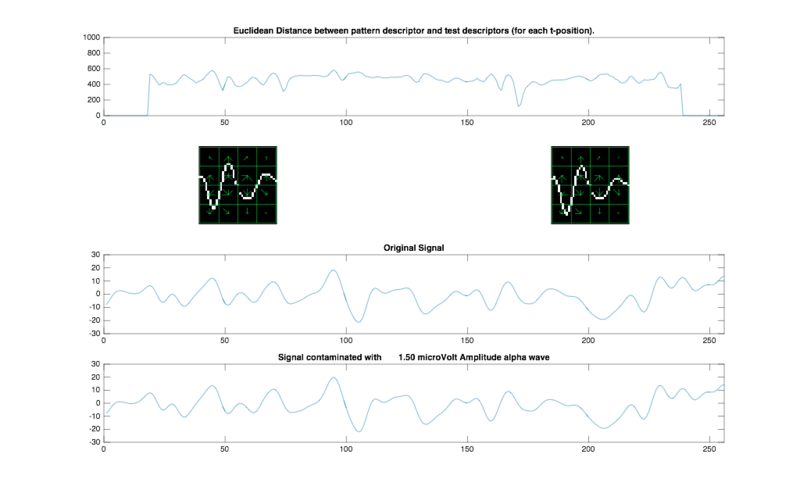
\includegraphics[scale=0.6]{images/dialdescriptores6.png}}
\caption[Dial Descriptors 1]{With a subtle $1.5 microvolt$ noisy $10 Hz$ signal, there isn't changes.}
\label{fig:dialdescriptors1}
\end{figure}


\begin{figure}[h!]
\centering
\subfigure[]
{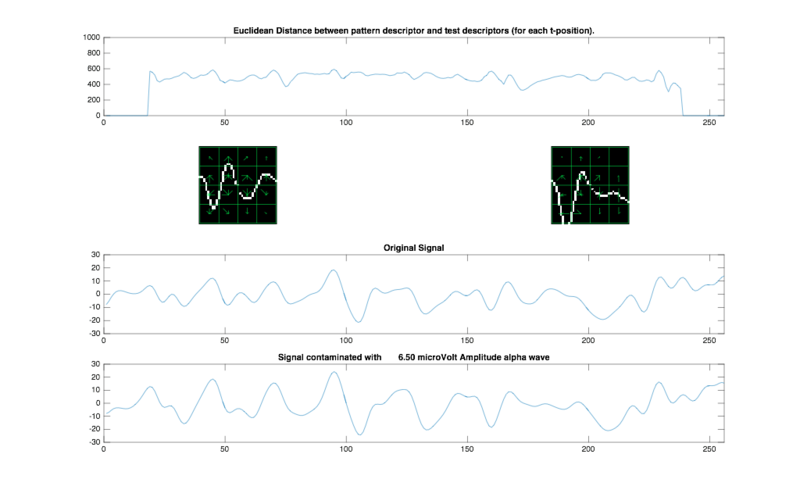
\includegraphics[scale=0.6]{images/dialdescriptores7.png}}
\caption[Dial Descriptors 1]{With a subtle $6.5 microvolt$ noisy $10 Hz$ signal, the keypoint cannot be localized at all.}
\label{fig:dialdescriptors1}
\end{figure}

